\documentclass[12pt,a4paper]{article}

% Packages
\usepackage[utf8]{inputenc}
\usepackage[margin=1in]{geometry}
\usepackage{graphicx}
\usepackage{hyperref}
\usepackage{amsmath}
\usepackage{amssymb}
\usepackage{algorithm}
\usepackage{algpseudocode}
\usepackage{booktabs}
\usepackage{xcolor}
\usepackage{listings}
\usepackage{caption}
\usepackage{subcaption}
\usepackage{tikz}
\usetikzlibrary{shapes,arrows,positioning}

% Hyperref setup
\hypersetup{
    colorlinks=true,
    linkcolor=blue,
    filecolor=magenta,      
    urlcolor=cyan,
    citecolor=blue
}

% Code listing setup
\lstset{
    basicstyle=\ttfamily\small,
    breaklines=true,
    frame=single,
    numbers=left,
    numberstyle=\tiny,
    commentstyle=\color{green!60!black},
    keywordstyle=\color{blue},
    stringstyle=\color{red}
}

% Title information
\title{\textbf{CC-ADOV: An Effective Multiple Paths Congestion Control AODV 
}}
\author{
    \textbf{Student Name:} Dipit Saha \\
    \textbf{Roll Number:} 2105050 
}

\date{\today}

\begin{document}

\maketitle

% \begin{abstract}
% Mobile Ad hoc Networks (MANETs) face significant challenges in maintaining Quality of Service (QoS) under congested network conditions. While the existing CC-AODV (Congestion Control AODV) protocol addresses congestion through a counter-based mechanism, it suffers from limitations including fixed threshold values, inefficient memory usage, and lack of dynamic adaptation to varying network loads. This project proposes an Enhanced CC-AODV (ECC-AODV) protocol that introduces adaptive threshold management, optimized packet header design, queue-length based congestion detection, and multi-metric path selection. The proposed enhancements aim to improve packet delivery ratio, reduce end-to-end delay, optimize memory usage, and provide better scalability in dense network scenarios. Implementation will be performed using NS-3 network simulator with comprehensive performance evaluation against both vanilla AODV and existing CC-AODV protocols.
% \end{abstract}

\newpage
\tableofcontents
\newpage

\section{Introduction}

\subsection{Background}
Mobile Ad hoc Networks (MANETs) are self-configuring networks of mobile devices connected wirelessly without requiring fixed infrastructure. These networks find applications in disaster relief, military operations, vehicular networks, and emergency response systems where traditional infrastructure is unavailable or impractical.

The Ad hoc On-Demand Distance Vector (AODV) routing protocol is one of the most widely deployed reactive routing protocols in MANETs. However, traditional AODV suffers from performance degradation under network congestion, as it always selects the shortest path without considering the load on intermediate nodes.

\subsection{Motivation}
Current challenges in MANET routing include:
\begin{itemize}
    \item \textbf{Congestion-blind routing:} Traditional AODV selects paths based solely on hop count, ignoring node congestion levels
    \item \textbf{Resource underutilization:} Some nodes remain idle while others are overloaded
    \item \textbf{Increased packet loss:} Congested nodes drop packets, degrading network performance
    \item \textbf{Higher delays:} Packets queue at busy nodes, increasing end-to-end delay
    \item \textbf{Poor scalability:} Performance degrades significantly as network density increases
\end{itemize}

\subsection{Project Scope}
This project focuses on enhancing the CC-AODV protocol to address its current limitations while maintaining backward compatibility with AODV and improving overall network performance.

\section{Literature Review}

\subsection{Paper 1: CC-AODV (Base Paper)}

\textbf{Title:} CC-ADOV: An Effective Multiple Paths Congestion Control AODV

\textbf{Authors:} Yefa Mai, Fernando Molina Rodriguez, and Dr. Nan Wang

\textbf{Published:} 2018 IEEE 8th Annual Computing and Communication Workshop and Conference (CCWC)

\textbf{Link:} \url{https://ieeexplore.ieee.org/document/8301758}

\textbf{DOI:} 10.1109/CCWC.2018.8301758

\subsubsection{Key Contributions}
\begin{enumerate}
    \item Introduced a \textbf{congestion counter} mechanism in the AODV routing table
    \item Added a \textbf{congestion flag} (32-bit) to RREP packet headers
    \item Implemented counter-based RREQ dropping at intermediate nodes
    \item Demonstrated improved packet delivery ratio and throughput in NS-3 simulations
\end{enumerate}

\subsubsection{How CC-AODV Works}
\begin{enumerate}
    \item \textbf{Route Discovery:}
    \begin{itemize}
        \item Source floods RREQ packets across the network
        \item Intermediate nodes check congestion counter against threshold
        \item If counter $<$ threshold: forward RREQ and update routing table
        \item If counter \geq threshold: drop RREQ (path too congested)
    \end{itemize}
    
    \item \textbf{Route Reply:}
    \begin{itemize}
        \item Destination generates RREP with congestion flag = true
        \item RREP unicasts back through intermediate nodes
        \item Each node checks congestion flag
        \item If flag = true: increment local congestion counter
        \item Update routing table with new route information
    \end{itemize}
    
    \item \textbf{Counter Management:}
    \begin{itemize}
        \item \textbf{Initialize:} Counter = 0 when routing table created
        \item \textbf{Increment:} Counter++ when RREP with congestion flag passes through
        \item \textbf{Decrement:} Counter-- when route lifetime expires or RERR sent
        \item \textbf{Reset:} Counter = 0 when node removed from network
    \end{itemize}
\end{enumerate}

% \subsubsection{Performance Results from Original Paper}
% \begin{table}[h]
% \centering
% \caption{CC-AODV vs AODV Performance Comparison}
% \begin{tabular}{@{}lccc@{}}
% \toprule
% \textbf{Metric} & \textbf{10 Nodes} & \textbf{30 Nodes} & \textbf{50 Nodes} \\ \midrule
% \textbf{PDR Improvement} & -0.46\% & +9.21\% & +0.57\% \\
% \textbf{Throughput Gain} & +22.66\% & +5.37\% & +12.39\% \\
% \textbf{Packet Loss Reduction} & +0.93\% & -7.68\% & -4.11\% \\
% \textbf{E2E Delay Change} & 0\% & +11.17\% & +25.39\% \\ \bottomrule
% \end{tabular}
% \end{table}

% \subsection{Paper 2: NetSim Implementation}

% \textbf{Title:} Congestion Control AODV (CC-AODV)

% \textbf{Source:} NetSim Standard v13.0 Implementation Guide

% \textbf{Link:} \url{https://github.com/NetSim-TETCOS/CC_AODV_Project_v13.0}

% \subsubsection{Implementation Details}
% The NetSim implementation provides:
% \begin{itemize}
%     \item Complete C source code modifications for AODV
%     \item Visual Studio 2019 project files
%     \item Sample network configurations (10 nodes, 30 nodes)
%     \item Performance comparison scripts
% \end{itemize}

% \subsubsection{Key Code Modifications}
% \begin{enumerate}
%     \item \textbf{RREP Structure (AODV.h):}
%     \begin{lstlisting}[language=C]
% struct stru_NetSim_AODV_RREP {
%     // ... existing fields ...
%     bool congestionflag : true;  // Added field
% };
%     \end{lstlisting}
    
%     \item \textbf{Device Variable (AODV.h):}
%     \begin{lstlisting}[language=C]
% struct stru_AODV_DeviceVariable {
%     // ... existing fields ...
%     unsigned int ncounter;  // Congestion counter
% };
%     \end{lstlisting}
    
%     \item \textbf{RREQ Processing (RREQ.c):}
%     \begin{lstlisting}[language=C]
% int dev_counter = AODV_DEV_VAR(nDeviceId)->ncounter;
% if (dev_counter > 25) {  // Fixed threshold!
%     fn_NetSim_Packet_FreePacket(packet);
%     return 1;  // Drop packet
% }
%     \end{lstlisting}
% \end{enumerate}

% \subsection{Related Work and Improvements}

% Several researchers have identified limitations and proposed improvements:

% \begin{enumerate}
%     \item \textbf{GitHub Implementation (kawshikbuet17):}
%     \begin{itemize}
%         \item Identified that 32-bit congestion flag is memory wasteful
%         \item Suggested using boolean variable instead
%         \item Noted that threshold value (25) requires careful tuning
%         \item Observed that congestion counter level significantly impacts PDR
%     \end{itemize}
    
%     \item \textbf{Congestion-Adaptive Routing Protocol (CRP):}
%     \begin{itemize}
%         \item Proposed dynamic route adaptation based on real-time congestion
%         \item Achieved 85\% improvement in E2E delay
%         \item Demonstrated 53.84\% improvement in PDR
%         \item Reduced routing overhead by 20.68\%
%     \end{itemize}
    
%     \item \textbf{Multi-Objective AOMDV:}
%     \begin{itemize}
%         \item Considers node quality and remaining energy
%         \item Selects routes based on multiple metrics
%         \item Maintains local lists of neighbor energy levels
%     \end{itemize}
% \end{enumerate}

\section{Problem Statement}

\subsection{Current Problems in CC-AODV}

Despite improvements over vanilla AODV, CC-AODV suffers from several critical limitations:

\begin{enumerate}
    \item \textbf{Fixed Threshold Problem:}
    \begin{itemize}
        \item Threshold value is hardcoded 
        \item Optimal threshold varies with network density and traffic load
        \item Fixed threshold performs poorly in dynamic scenarios
        \item No mechanism to adapt threshold based on network conditions
    \end{itemize}
    
    \item \textbf{Inefficient Memory Usage:}
    \begin{itemize}
        \item Uses 32-bit field for boolean congestion flag (wasteful)
        \item Adds overhead to every RREP packet (4 bytes per packet)
        \item No compression or optimization of routing table entries
    \end{itemize}
    
    \item \textbf{Crude Congestion Detection:}
    \begin{itemize}
        \item Only counts number of routes passing through node
        \item Ignores actual queue length and packet processing rate
        \item Does not consider buffer occupancy or channel utilization
        \item Binary flag (congested/not congested) lacks granularity
    \end{itemize}
    
    \item \textbf{Lack of Path Diversity:}
    \begin{itemize}
        \item Still selects single path based on counter comparison
        \item Does not maintain alternative routes
        \item No load balancing across multiple available paths
        \item Cannot adapt if selected path becomes congested mid-transmission
    \end{itemize}
    
    \item \textbf{Higher End-to-End Delay:}
    \begin{itemize}
        \item Selecting longer (less congested) paths increases hop count
        \item Additional processing overhead from counter checks
        \item Delay increases significantly in dense networks (25\% increase at 50 nodes)
    \end{itemize}
    
    \item \textbf{Limited Scalability:}
    \begin{itemize}
        \item Performance degrades in very dense networks 
        \item Control overhead increases with network size
        \item No differentiation between traffic types (UDP vs TCP)
    \end{itemize}
\end{enumerate}

% \subsection{Research Questions}

% This project aims to answer the following questions:

% \begin{enumerate}
%     \item Can we develop an adaptive threshold mechanism that adjusts based on real-time network conditions?
%     \item How can we optimize memory usage while maintaining congestion awareness?
%     \item What metrics beyond simple counter values can improve congestion detection accuracy?
%     \item Can we reduce end-to-end delay while maintaining congestion avoidance benefits?
%     \item How can we improve scalability for larger, denser networks?
% \end{enumerate}

\section{Proposed Solution: ECC-AODV}

\subsection{Overview}

Enhanced CC-AODV (ECC-AODV) introduces four major improvements:

\begin{enumerate}
    \item \textbf{Adaptive Threshold Management (ATM)}
    \item \textbf{Queue-Aware Congestion Detection (QACD)}
    \item \textbf{Optimized Packet Header Design (OPHD)}
    % \item \textbf{Multi-Metric Path Selection (MMPS)}
\end{enumerate}

\subsection{Modification 1: Adaptive Threshold Management (ATM)}

\subsubsection{Concept}
Instead of using a fixed threshold value, ATM dynamically adjusts the congestion threshold based on:
\begin{itemize}
    \item Current network density (number of active nodes)
    \item Average congestion level across all nodes
    \item Packet delivery ratio trends
    \item Traffic intensity
\end{itemize}

% \subsubsection{Algorithm}

% \begin{algorithm}
% \caption{Adaptive Threshold Calculation}
% \begin{algorithmic}[1]
% \State $N \gets$ total number of nodes in network
% \State $avg\_counter \gets$ average congestion counter across all neighbors
% \State $pdr \gets$ current packet delivery ratio
% \State $base\_threshold \gets 25$ \Comment{Starting point}
% \State
% \If{$N \leq 10$}
%     \State $threshold \gets base\_threshold \times 0.6$ \Comment{Small network}
% \ElsIf{$N \leq 30$}
%     \State $threshold \gets base\_threshold \times 1.0$ \Comment{Medium network}
% \Else
%     \State $threshold \gets base\_threshold \times 1.4$ \Comment{Large network}
% \EndIf
% \State
% \State $threshold \gets threshold \times (1 + \frac{avg\_counter}{100})$ \Comment{Adjust for congestion}
% \State
% \If{$pdr < 0.5$}
%     \State $threshold \gets threshold \times 0.8$ \Comment{Network stressed, be more selective}
% \ElsIf{$pdr > 0.8$}
%     \State $threshold \gets threshold \times 1.2$ \Comment{Network healthy, be more permissive}
% \EndIf
% \State
% \State \Return $\lfloor threshold \rfloor$
% \end{algorithmic}
% \end{algorithm}

\subsubsection{Benefits}
\begin{itemize}
    \item Adapts to varying network sizes automatically
    \item Responds to network stress in real-time
    \item Prevents overly restrictive routing in low-traffic scenarios
    \item Maintains effectiveness in high-traffic scenarios
\end{itemize}

\subsection{Modification 2: Queue-Aware Congestion Detection (QACD)}

\subsubsection{Concept}
Instead of relying solely on route counter, QACD incorporates actual queue measurements:
\begin{itemize}
    \item Current queue length (number of packets in buffer)
    \item Queue occupancy percentage
    \item Packet drop rate at the queue
    \item Average waiting time in queue
\end{itemize}

\subsubsection{Congestion Level Formula}

\begin{equation}
CL = w_1 \times \frac{Q_{current}}{Q_{max}} + w_2 \times \frac{Counter}{Threshold} + w_3 \times DropRate
\end{equation}

Where:
\begin{itemize}
    \item $CL$ = Congestion Level (0 to 1)
    \item $Q_{current}$ = Current queue length
    \item $Q_{max}$ = Maximum queue capacity
    \item $Counter$ = Current congestion counter value
    \item $Threshold$ = Dynamic threshold from ATM
    \item $DropRate$ = Recent packet drop rate (0 to 1)
    \item $w_1, w_2, w_3$ = Weights (must sum to 1.0)
\end{itemize}

% \textbf{Recommended weights:} $w_1 = 0.5$, $w_2 = 0.3$, $w_3 = 0.2$

\subsubsection{Decision Making}

\begin{algorithm}
\caption{QACD-based Route Decision}
\begin{algorithmic}[1]
\State $CL \gets$ Calculate congestion level using Equation 1
\State
\If{$CL < 0.3$}
    \State \Return \textsc{Low Congestion} \Comment{Accept and forward RREQ}
\ElsIf{$CL < 0.7$}
    \State \Return \textsc{Moderate Congestion} \Comment{Accept but mark in RREP}
\Else
    \State \Return \textsc{High Congestion} \Comment{Drop RREQ}
\EndIf
\end{algorithmic}
\end{algorithm}

\subsection{Modification 3: Optimized Packet Header Design (OPHD)}

\subsubsection{Problem}
Original CC-AODV uses 32-bit field for boolean flag. 31 wasted bits per packet!

\subsubsection{Solution}
\begin{enumerate}
    \item \textbf{Use a 2-bit congestion level field} instead of a 32-bit boolean:
    \begin{itemize}
        \item 00 = No congestion ($CL < 0.3$)
        \item 01 = Low congestion ($0.3 \leq CL < 0.5$)
        \item 10 = Moderate congestion ($0.5 \leq CL < 0.7$)
        \item 11 = High congestion ($CL \geq 0.7$)
    \end{itemize}


    \item \textbf{Add 4-bit hop quality metric:}
    \begin{itemize}
        \item Encodes average queue occupancy along path
        \item Allows source to select best among multiple RREPs
        \item Values 0-15 representing 0\%-100\% occupancy
    \end{itemize}
    
    \item \textbf{Result:} Total 6 bits instead of 32 bits
    \begin{itemize}
        \item Memory savings: 81.25\% per RREP packet
        \item More granular congestion information
        \item Supports path quality comparison
    \end{itemize}
\end{enumerate}

\subsubsection{New RREP Header Structure}

% \begin{lstlisting}[language=C]
% struct ECC_AODV_RREP {
%     // ... existing AODV fields ...
    
%     unsigned int congestion_level:2;    // 0-3 (2 bits)
%     unsigned int path_quality:4;        // 0-15 (4 bits)
%     unsigned int reserved:10;           // For future use
    
%     // Total: 16 bits instead of 32 bits
% };
% \end{lstlisting}

\subsection{Modification 4: Multi-Metric Path Selection (MMPS)}

\subsubsection{Concept}
Source node receives multiple RREPs and selects best path based on multiple criteria:

\begin{enumerate}
    \item Hop count (lower is better)
    \item Cumulative congestion level (lower is better)
    \item Path quality metric (higher is better)
    \item Route freshness (sequence number)
\end{enumerate}

\subsubsection{Path Score Formula}

\begin{equation}
Score = \alpha \times \frac{1}{HopCount} + \beta \times PathQuality + \gamma \times \frac{1}{CongestionLevel + 1}
\end{equation}

Where:
\begin{itemize}
    \item $\alpha = 0.3$ (hop count weight)
    \item $\beta = 0.4$ (path quality weight)
    \item $\gamma = 0.3$ (congestion avoidance weight)
\end{itemize}

\textbf{Select path with highest score.}

\subsubsection{Algorithm}

\begin{algorithm}
\caption{Multi-Metric Path Selection}
\begin{algorithmic}[1]
\State $paths \gets$ all received RREPs for destination
\State $best\_path \gets null$
\State $best\_score \gets 0$
\State
\For{each $path$ in $paths$}
    \State $hop\_score \gets \alpha / path.hop\_count$
    \State $quality\_score \gets \beta \times (path.path\_quality / 15)$
    \State $congestion\_score \gets \gamma / (path.congestion\_level + 1)$
    \State
    \State $total\_score \gets hop\_score + quality\_score + congestion\_score$
    \State
    \If{$total\_score > best\_score$}
        \State $best\_score \gets total\_score$
        \State $best\_path \gets path$
    \EndIf
\EndFor
\State
\State \Return $best\_path$
\end{algorithmic}
\end{algorithm}

\subsection{Complete ECC-AODV Algorithm Flow}
\begin{figure}[h]
\centering
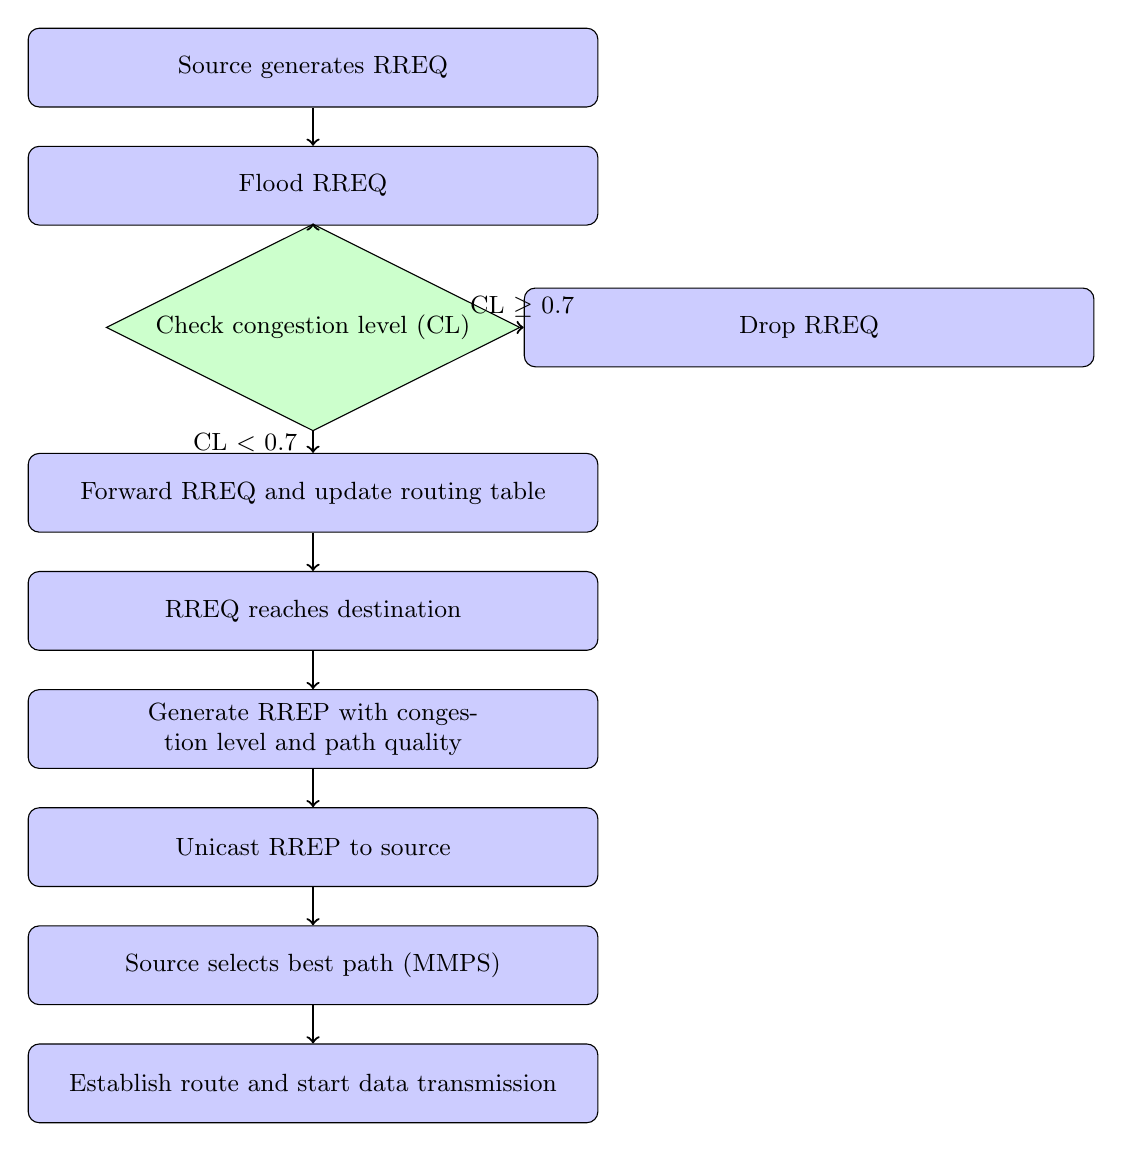
\begin{tikzpicture}[
    node distance=1.5cm,
    every node/.style={font=\small},
    block/.style={
        rectangle,
        draw,
        fill=blue!20,
        text width=7cm,
        text centered,
        rounded corners,
        minimum height=1cm
    },
    decision/.style={
        diamond,
        draw,
        fill=green!20,
        text width=4.2cm,
        text centered,
        aspect=2,
        inner sep=2pt
    },
    arrow/.style={->, thick}
]

% Nodes
\node[block] (rreq) {Source generates RREQ};
\node[block, below of=rreq] (flood) {Flood RREQ};

\node[decision, below of=flood, yshift=-0.3cm] (check)
{Check congestion level (CL)};

\node[block, below of=check, yshift=-0.6cm] (forward)
{Forward RREQ and update routing table};

\node[block, right of=check, xshift=4.8cm] (drop)
{Drop RREQ};

\node[block, below of=forward] (dest)
{RREQ reaches destination};

\node[block, below of=dest] (rrep)
{Generate RREP with congestion level and path quality};

\node[block, below of=rrep] (unicast)
{Unicast RREP to source};

\node[block, below of=unicast] (select)
{Source selects best path (MMPS)};

\node[block, below of=select] (route)
{Establish route and start data transmission};

% Arrows
\draw[arrow] (rreq) -- (flood);
\draw[arrow] (flood) -- (check);

\draw[arrow] (check) -- node[left, xshift=-2pt]{CL $<$ 0.7} (forward);
\draw[arrow] (check.east) -- node[midway, above]{CL $\ge$ 0.7} (drop.west);

\draw[arrow] (forward) -- (dest);
\draw[arrow] (dest) -- (rrep);
\draw[arrow] (rrep) -- (unicast);
\draw[arrow] (unicast) -- (select);
\draw[arrow] (select) -- (route);

\end{tikzpicture}
\caption{ECC-AODV Protocol Flow}
\label{fig:ecc-aodv-flow}
\end{figure}


\section{Challenges and Mitigation}

\subsection{Technical Challenges}

\begin{enumerate}
    \item \textbf{Challenge:} Balancing multiple metrics in path selection
    \begin{itemize}
        \item \textbf{Mitigation:} Extensive testing to tune weights ($\alpha$, $\beta$, $\gamma$)
        \item Use machine learning for weight optimization (future work)
    \end{itemize}
    
    \item \textbf{Challenge:} Overhead of queue monitoring
    \begin{itemize}
        \item \textbf{Mitigation:} Periodic sampling instead of continuous monitoring
        \item Use lightweight queue statistics already maintained by NS-3
    \end{itemize}
    
    \item \textbf{Challenge:} Increased computation for adaptive threshold
    \begin{itemize}
        \item \textbf{Mitigation:} Update threshold only periodically (every 5s)
        \item Use efficient moving average algorithms
    \end{itemize}
    
    \item \textbf{Challenge:} Backward compatibility with vanilla AODV
    \begin{itemize}
        \item \textbf{Mitigation:} Use reserved bits in AODV header
        \item Ensure graceful degradation when ECC-AODV nodes communicate with AODV nodes
    \end{itemize}
\end{enumerate}


\section{Future Work}

\subsection{Potential Extensions}

\begin{enumerate}
    \item \textbf{Machine Learning Integration:}
    \begin{itemize}
        \item Use ML to predict congestion before it occurs
        \item Optimize weight parameters automatically
        \item Anomaly detection for malicious nodes
    \end{itemize}
    
    \item \textbf{Energy Awareness:}
    \begin{itemize}
        \item Incorporate remaining battery levels in path selection
        \item Balance between congestion avoidance and energy efficiency
    \end{itemize}
    
    \item \textbf{QoS Support:}
    \begin{itemize}
        \item Differentiate paths based on traffic type (voice, video, data)
        \item Implement priority-based routing
    \end{itemize}
    
    \item \textbf{Security Enhancements:}
    \begin{itemize}
        \item Detect nodes falsely reporting congestion
        \item Implement authentication for routing messages
    \end{itemize}
    
  
\end{enumerate}


\section*{References}

\begin{enumerate}
    \item Y. Mai, F. M. Rodriguez and N. Wang, "CC-ADOV: An effective multiple paths congestion control AODV," 2018 IEEE 8th Annual Computing and Communication Workshop and Conference (CCWC), Las Vegas, NV, USA, 2018, pp. 1000-1004. doi: 10.1109/CCWC.2018.8301758
    
%     \item NetSim TETCOS, "Congestion Control AODV (CC-AODV) - NetSim v13.0," Available: \url{https://github.com/NetSim-TETCOS/CC_AODV_Project_v13.0}
    
%     \item Kawshik BUET, "Congestion-Control-AODV Implementation and Analysis," Available: \url{https://github.com/kawshikbuet17/Congestion-Control-AODV}
    
%     \item C. Perkins, E. Belding-Royer, and S. Das, "Ad hoc On-Demand Distance Vector (AODV) Routing," RFC 3561, July 2003.
    
%     \item NS-3 Consortium, "NS-3 Network Simulator Documentation," Available: \url{https://www.nsnam.org/documentation/}
    
%     \item S. Basagni et al., "Mobile Ad Hoc Networks: The Cutting Edge Directions," IEEE Press, 2004.
    
%     \item I. Chlamtac and A. Farago, "Making transmission schedules immune to topology changes in multi-hop packet radio networks," IEEE/ACM Trans. Networking, vol. 2, no. 1, pp. 23-29, Feb. 1994.
    
%     \item D. Johnson, Y. Hu, and D. Maltz, "The Dynamic Source Routing Protocol (DSR) for Mobile Ad Hoc Networks for IPv4," RFC 4728, Feb. 2007.
\end{enumerate}


\end{document}